\documentclass[handout]{beamer}  
%use [handout] option to print without all the pauses!
\usepackage{setspace}
\linespread{1.3}
\usepackage{amssymb, amsmath, amsthm} 
\usepackage{rotating}
\usepackage{multirow}
\usepackage{graphicx}
\usepackage{enumerate}
\usepackage{synttree}
\usepackage{fancybox}
\usepackage{color}
\usepackage{tikz}
\usetikzlibrary{trees}
\newcommand{\p}{\mathbb{P}}
\newcommand{\expect}{\mathbb{E}}
\newcommand{\var}{\mathbb{V}}



%\setbeamertemplate{blocks}[rounded][shadow=true] 
%gets rid of bottom navigation bars
\setbeamertemplate{footline}{
   \begin{beamercolorbox}[ht=4ex,leftskip=0.3cm,rightskip=0.3cm]{author in head/foot}
%    \usebeamercolor{UniBlue}
    \vspace{0.1cm}
    %\insertshorttitle \ - \insertdate 
    \hfill \insertframenumber / \inserttotalframenumber
   \end{beamercolorbox}
   \vspace*{0.1cm}
} 

%gets rid of navigation symbols
\setbeamertemplate{navigation symbols}{}


%Include or exclude the notes?
%\setbeameroption{show notes}
\setbeameroption{hide notes}


\title[Econ 103]{Economics 103, Statistics for Economists} 
\author[F. DiTraglia]{Francis J.\ DiTraglia}
\institute{University of Pennsylvania}
\date{Lecture 17}


\begin{document} 




%%%%%%%%%%%%%%%%%%%%%%%%%%%%%%%%%%%%%%%%

\begin{frame}[plain]
	\titlepage 
	

\end{frame} 



%%%%%%%%%%%%%%%%%%%%%%%%%%%%%%%%%%%%%%%%


\begin{frame}
\begin{block}{Last Time}
Confidence Interval for Population Mean:
$$\boxed{\bar{X}_n \pm \texttt{qnorm}(1-\alpha/2) \times \sigma/\sqrt{n}}$$
Based on Assumptions:
	\begin{enumerate}
\item The population standard deviation $\sigma$ was known.
\item The population is normally distributed (bell-shaped).
\end{enumerate}
\end{block}
\begin{block}{Today}
What if population is normal but $\sigma$ is unknown?
\end{block}

\end{frame}
%%%%%%%%%%%%%%%%%%%%%%%%%%%%%%%%%%%%%%%%
\begin{frame}
\frametitle{We Don't know $\sigma$. What to use instead?}
$$\boxed{\bar{X}_n \pm \texttt{qnorm}(1-\alpha/2) \times \sigma/\sqrt{n}}$$

\begin{block}{What about Sample Standard Deviation $S$?}
	$$\p\left(-2 \leq \frac{\bar{X}_n-\mu}{S/\sqrt{n}} \leq 2 \right) = 0.95 \mbox{ ???}$$
\end{block}

\begin{block}{Not Quite!}
Although $(\bar{X}_n-\mu)/(\sigma/\sqrt{n})\sim N(0,1)$, $S \neq \sigma$. In fact, $S$ is an \alert{estimator} of $\sigma$ so it is a \alert{random variable!}
\end{block}
\end{frame}
%%%%%%%%%%%%%%%%%%%%%%%%%%%%%%%%%%%%%%%%

\begin{frame}
\frametitle{What is the sampling distribution?}
Suppose $X_1, \hdots, X_n \sim N(\mu,\sigma^2)$
 $$\boxed{\frac{\bar{X}_n-\mu}{S/\sqrt{n}}  \sim \mbox{ ???}}$$

 \begin{block}{First Step}
What is the sampling distribution of $S$?
\end{block}
\end{frame}
%%%%%%%%%%%%%%%%%%%%%%%%%%%%%%%%%%%%%%%%
\begin{frame}
\frametitle{What is the Distribution? \hfill 
\includegraphics[scale = 0.05]{./images/clicker}}
Suppose $X_1, \hdots, X_n \sim N(\mu,\sigma^2)$. What is the distribution of this sum?
	$$\sum_{i=1}^n \left(\frac{X_i - \mu}{\sigma}\right)^2$$
	
	\begin{enumerate}[(a)]
\item $\chi^2(n)$
\item $N(\mu, \sigma^2)$
\item $N(0,1)$
\item $N(\mu, \sigma^2/n)$
\item $\chi^2(1)$
\end{enumerate}
\end{frame}
%%%%%%%%%%%%%%%%%%%%%%%%%%%%%%%%%%%%%%%%
\begin{frame}
\frametitle{Towards the Sampling Dist.\ of $S$}
If $X_1, \hdots, X_n \sim N(\mu,\sigma^2)$, then 
$$\sum_{i=1}^n \left(\frac{X_i - \mu}{\sigma}\right)^2 \sim \chi^2(n)$$

Now:
$$\sum_{i=1}^n \left(\frac{X_i - \mu}{\sigma}\right)^2   = \pause \left(\frac{n-1}{\sigma^2}\right) \left[\frac{1}{n-1}\sum_{i=1}^n \left(X_i - \mu\right)^2\right] \pause \sim \chi^2(n) $$
\alert{Anything look familiar?}
\end{frame}
%%%%%%%%%%%%%%%%%%%%%%%%%%%%%%%%%%%%%%%%

\begin{frame}
\frametitle{Sampling Distribution of Sample Variance}
Suppose $X_1, \hdots, X_n \sim N(\mu,\sigma^2)$. Then whereas
$$\left(\frac{n-1}{\sigma^2}\right) \left[\frac{1}{n-1}\sum_{i=1}^n \left(X_i - \mu\right)^2\right] \sim \chi^2(n)$$
\pause
Replacing $\mu$ with $\bar{X}$ ``loses'' a degree of freedom
	$$\left(\frac{n-1}{\sigma^2}\right) \left[\frac{1}{n-1}\sum_{i=1}^n \left(X_i - \bar{X}\right)^2\right] =\pause\alert{ \left(\frac{n-1}{\sigma^2}\right)S^2} \pause \alert{\sim \chi^2(n-1)}$$


\alert{Ultimately, we will use this fact to work out the sampling distribution of $\sqrt{n}(\bar{X}_n-\mu)/S$, but for now let's take a detour...}
\end{frame}
%%%%%%%%%%%%%%%%%%%%%%%%%%%%%%%%%%%%%%%%
\begin{frame}
\frametitle{95\% CI for Variance of Normal Population}
We know that:
	$$\left( \frac{n-1}{\sigma^2}\right)S^2\sim \chi^2(n-1)$$
	\pause
	\vspace{2em}
	
First Step: find $a,b$ such that 
	$$\p\left[ a\leq   \left( \frac{n-1}{\sigma^2}\right)S^2 \leq b \right] = 0.95$$
	\pause
\alert{Although there are many choices for $a,b$ that would work, a sensible idea is to put 2.5\% in each tail...}
\end{frame}
%%%%%%%%%%%%%%%%%%%%%%%%%%%%%%%%%%%%%%%%
\begin{frame}
\begin{figure}
\centering
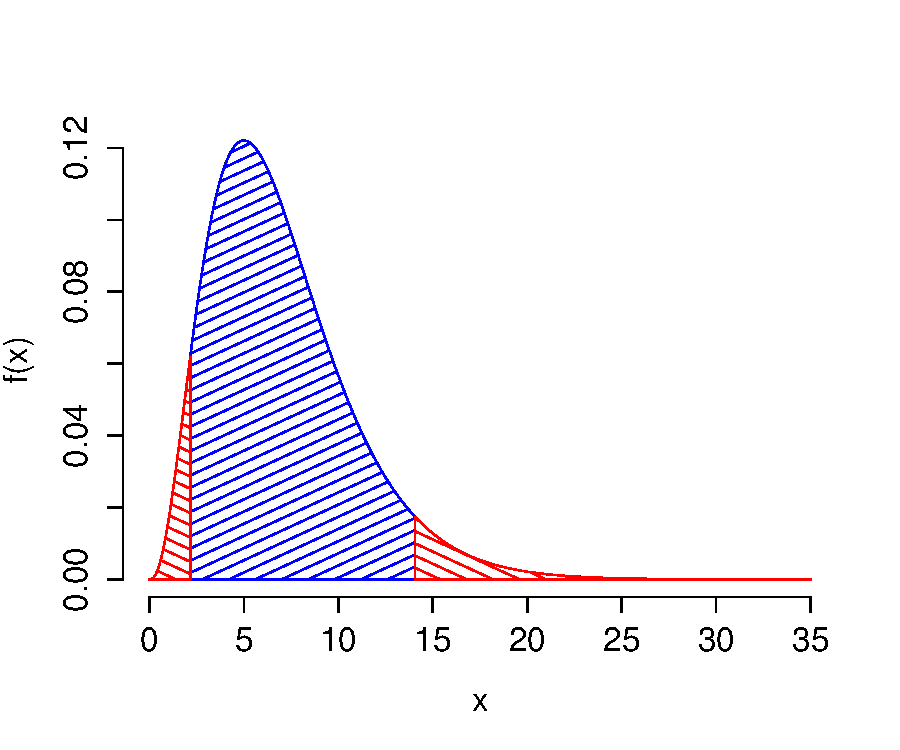
\includegraphics[scale = 0.65]{./images/chisq_tails}
\end{figure}
\end{frame}
%%%%%%%%%%%%%%%%%%%%%%%%%%%%%%%%%%%%%%%%
\begin{frame}
\frametitle{What R command should I use to calculate $a$? \hfill 
\includegraphics[scale = 0.05]{./images/clicker}}
$$P\left[ a\leq   \left( \frac{n-1}{\sigma^2}\right)S^2 \leq b \right] = 0.95$$
	\begin{enumerate}[(a)]
		\item \texttt{qchisq}$( 0.95, \texttt{df = } n-1)$
		\item \texttt{qchisq}$( 0.025, \texttt{df = }  n)$
		\item \texttt{qchisq}$(0.975, \texttt{df = }  n-1)$
		\item \texttt{qchisq}$( 0.025, \texttt{df = }  n-1)$
		\item \texttt{qchisq}$(0.975, \texttt{df = }  n)$
	\end{enumerate}
\end{frame}
%%%%%%%%%%%%%%%%%%%%%%%%%%%%%%%%%%%%%%%%
\begin{frame}
\frametitle{What R command should I use to calculate $b$? \hfill 
\includegraphics[scale = 0.05]{./images/clicker}}
$$P\left[ a\leq   \left( \frac{n-1}{\sigma^2}\right)S^2 \leq b \right] = 0.95$$
	\begin{enumerate}[(a)]
		\item \texttt{qchisq}$( 0.95, \texttt{df = } n-1)$
		\item \texttt{qchisq}$( 0.025, \texttt{df = }  n)$
		\item \texttt{qchisq}$(0.975, \texttt{df = }  n-1)$
		\item \texttt{qchisq}$( 0.025, \texttt{df = }  n-1)$
		\item \texttt{qchisq}$(0.975, \texttt{df = }  n)$
	\end{enumerate}
\end{frame}
%%%%%%%%%%%%%%%%%%%%%%%%%%%%%%%%%%%%%%%%
\begin{frame}
\begin{figure}
\centering
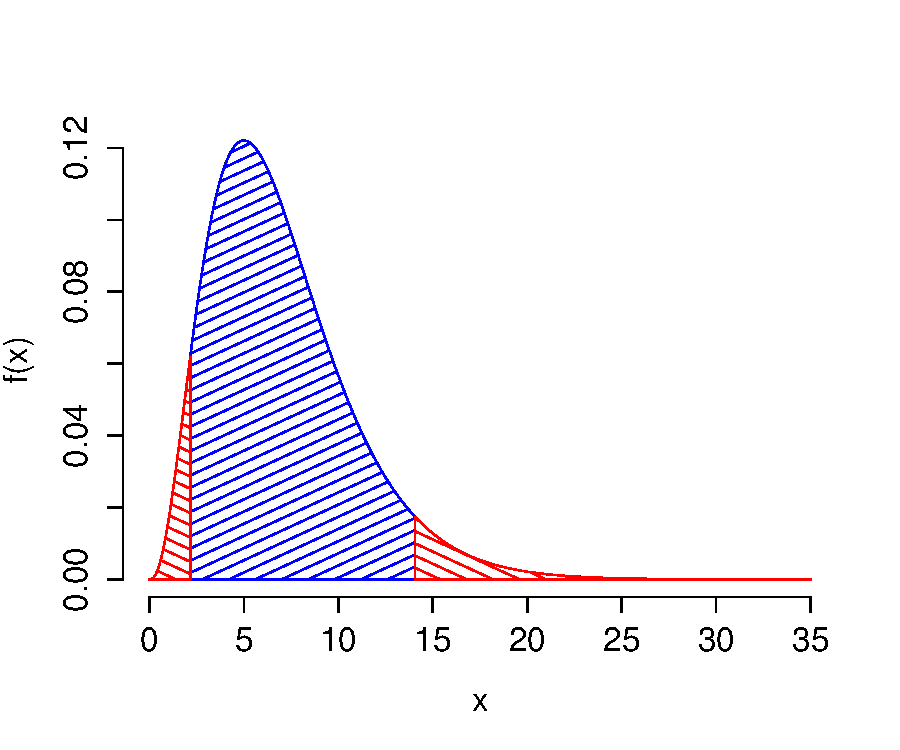
\includegraphics[scale = 0.55]{./images/chisq_tails}
\end{figure}

a = \texttt{qchisq(0.025, df = n - 1)} \\

b = \texttt{qchisq(0.975, df = n - 1)} 
\end{frame}
%%%%%%%%%%%%%%%%%%%%%%%%%%%%%%%%%%%%%%%%

\begin{frame}
\frametitle{Step 2: After Finding $a,b$ Rearrange}
 	\begin{eqnarray*}
 		P\left[ a\leq   \left( \frac{n-1}{\sigma^2}\right)S^2 \leq b \right] &=& 0.95 \\ \\ \pause
 		P\left[ \frac{a}{(n-1)S^2}\leq  \frac{1}{\sigma^2} \leq \frac{b}{(n-1)S^2} \right] &=& 0.95 \\ \\ \pause
 				P\left[ \frac{(n-1)S^2}{b}\leq  \sigma^2 \leq \frac{(n-1)S^2}{a} \right] &=& 0.95
 	\end{eqnarray*}	
 	\pause
\alert{This CI is \emph{not} symmetric: it \emph{doesn't} take the form $\widehat{\theta} \pm ME$!}
\end{frame}
%%%%%%%%%%%%%%%%%%%%%%%%%%%%%%%%%%%%%%%%
\begin{frame}
\frametitle{Example: 95\% Confidence Interval for Normal Variance}
$X_1, \hdots, X_{100} \sim N(\mu,\sigma^2)$. Here $n-1 = 99$, hence \pause
	\begin{eqnarray*}
		a = \texttt{qchisq(0.025, df = 99)} &\approx& 73\\ \pause
		b = \texttt{qchisq(0.975, df = 99)} &\approx& 128 \pause
	\end{eqnarray*}	
From the sample data, $s^2 = 4.3$
	\begin{eqnarray*}
		LCL &=& (n-1)s^2/b = \pause 99 \times 4.3/128 \pause \approx 3.3\\ \pause
		UCL &=& (n-1)s^2/a = \pause 99 \times 4.3/73 \pause \approx  5.8
	\end{eqnarray*}
	\pause
	\alert{95\% CI for $\sigma^2$ is $[3.3, 5.8]$. What values are plausible?}\\
	\pause
	The actual population variance in this case was 4
\end{frame}
%%%%%%%%%%%%%%%%%%%%%%%%%%%%%%%%%%%%%%%%
\begin{frame}
\frametitle{Arbitrary Confidence Level: $(1-\alpha)$}

\begin{figure}
\centering
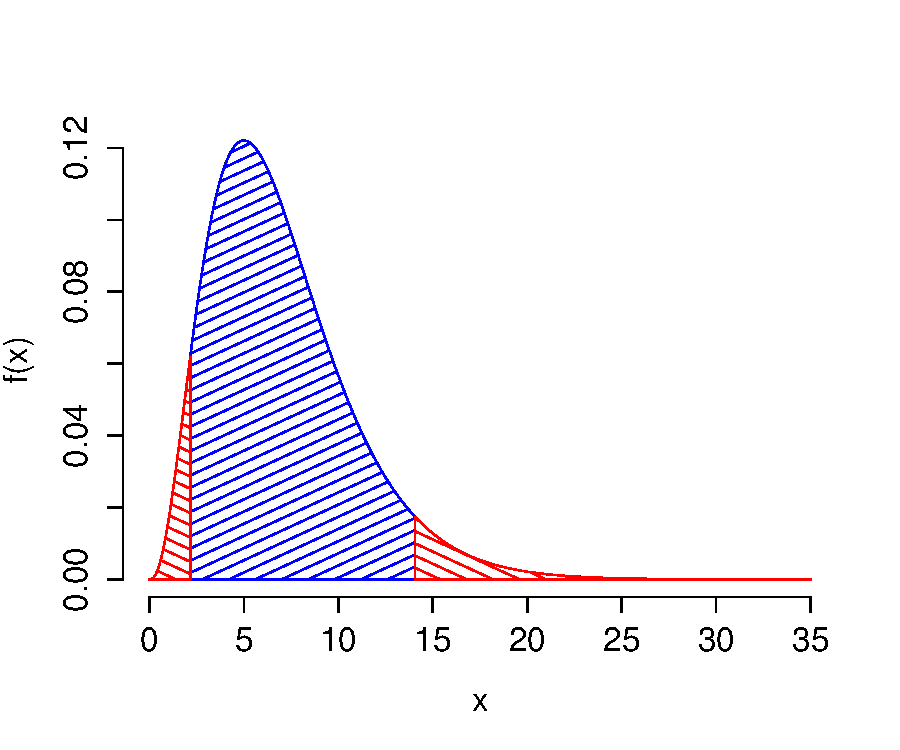
\includegraphics[scale = 0.5]{./images/chisq_tails}
\end{figure}

a = \texttt{qchisq($\alpha/2$, df = n - 1)} \\

b = \texttt{qchisq($1-\alpha/2$, df = n - 1)} 
\end{frame}
%%%%%%%%%%%%%%%%%%%%%%%%%%%%%%%%%%%%%%%%
\begin{frame}
\frametitle{CI for Normal Variance}
a = \texttt{qchisq($\alpha/2$, df = n - 1)} \\
b = \texttt{qchisq($1-\alpha/2$, df = n - 1)} 
\vspace{1em}
 	\begin{eqnarray*}
 		P\left[ a\leq   \left( \frac{n-1}{\sigma^2}\right)S^2 \leq b \right] &=& 1-\alpha \\ \\
 		P\left[ \frac{a}{(n-1)S^2}\leq  \frac{1}{\sigma^2} \leq \frac{b}{(n-1)S^2} \right] &=& 1-\alpha \\ \\ 
 				P\left[ \frac{(n-1)S^2}{b}\leq  \sigma^2 \leq \frac{(n-1)S^2}{a} \right] &=& 1-\alpha
 	\end{eqnarray*}	
\end{frame}
%%%%%%%%%%%%%%%%%%%%%%%%%%%%%%%%%%%%%%%%
\begin{frame}
\frametitle{CI for Normal Variance}
Suppose $X_1, \hdots, X_n \sim \mbox{iid } N(\mu,\sigma^2)$ and let:
	\begin{eqnarray*}
		a &=& \texttt{qchisq($\alpha/2$, df = n - 1)} \\
		b &=& \texttt{qchisq($1-\alpha/2$, df = n - 1)} 
	\end{eqnarray*}
Then,
	$$\left[ \frac{(n-1)S^2}{b}, \frac{(n-1)S^2}{a} \right]$$
is a $100\times(1-\alpha)\%$ confidence interval for $\sigma^2$.
\end{frame}
%%%%%%%%%%%%%%%%%%%%%%%%%%%%%%%%%%%%%%%%
\begin{frame}
\frametitle{End of Detour}
We want to know the Sampling Distribution of $\sqrt{n}(\bar{X}_n - \mu)/S$ and we just saw that:
$$\boxed{\left( \frac{n-1}{\sigma^2}\right)S^2\sim \chi^2(n-1)}$$
\begin{alertblock}{How can we use this fact to help us?}
\end{alertblock}
\end{frame}
%%%%%%%%%%%%%%%%%%%%%%%%%%%%%%%%%%%%%%%%
\begin{frame}
\frametitle{What is the Sampling Distribution of $\sqrt{n}(\bar{X}_n-\mu)/S$?}
This slide is just algebra:
\begin{eqnarray*}
	\frac{\bar{X}_n - \mu}{S/\sqrt{n}} &=&\pause \frac{\bar{X}_n - \mu}{S/\sqrt{n}} \cdot \left(\frac{\sigma/\sqrt{n}}{\sigma/\sqrt{n}} \right) = \pause \left(\frac{\bar{X}_n - \mu}{\alert{\sigma/\sqrt{n}}} \right)\left(\frac{\sigma/\sqrt{n}}{\alert{S/\sqrt{n}}} \right)\\ \\
	&=& \pause\left(\frac{\bar{X}_n - \mu}{\sigma/\sqrt{n}} \right)\left(\frac{\sigma}{S} \right) = \pause  \left(\frac{\bar{X}_n - \mu}{\sigma/\sqrt{n}} \right)\left(\sqrt{\frac{n-1}{n-1}}\cdot\sqrt{\frac{\sigma^2}{S^2}} \right) \\ \\
	&=& \pause \left(\frac{\bar{X}_n - \mu}{\sigma/\sqrt{n}} \right)\left(\sqrt{\frac{(n-1)\sigma^2}{(n-1)S^2}} \right) \\ \\
	&=& \pause \frac{\displaystyle \left(\frac{\bar{X}_n - \mu}{\sigma/\sqrt{n}}\right)}{\sqrt{\left[\frac{(n-1)S^2}{\sigma^2}\right]/(n-1)}} 
\end{eqnarray*}
\end{frame}
%%%%%%%%%%%%%%%%%%%%%%%%%%%%%%%%%%%%%%%%
\begin{frame}[t]\frametitle{Distribution of $\sqrt{n}(\bar{X}_n - \mu)/\sigma$ \hfill 
\includegraphics[scale = 0.05]{./images/clicker}}
    
    Suppose $X_1, \hdots, X_n \sim \mbox{ iid } N(\mu, \sigma^2)$ and $\bar{X}_n$ is ths sample mean. Then the sampling distribution of \alert{$\sqrt{n}(\bar{X}_n - \mu)/\sigma$} is

    \begin{enumerate}[(a)]
    	\item $t(n)$
    	\item $t(n-1)$
    	\item $\chi^2(n)$
    	\item $\chi^2(n-1)$
    	\item $N(\mu, \sigma^2)$
    	\item $N(0,1)$
    	\item $N(\mu, \sigma^2/n)$
    	\item $F(n, n-1)$
    \end{enumerate}


\end{frame}
%%%%%%%%%%%%%%%%%%%%%%%%%%%%%%%%%%%%%%%%
\begin{frame}[c]\frametitle{Distribution of $(n-1)S^2/\sigma^2$ \hfill 
\includegraphics[scale = 0.05]{./images/clicker}}
    
    Suppose $X_1, \hdots, X_n \sim \mbox{ iid } N(\mu, \sigma^2)$ and $S^2$ is the sample variance. Then the sampling distribution of \alert{$(n-1)S^2/\sigma^2$} is

    \begin{enumerate}[(a)]
    	\item $t(n)$
    	\item $t(n-1)$
    	\item $\chi^2(n)$
    	\item $\chi^2(n-1)$
    	\item $N(\mu, \sigma^2)$
    	\item $N(0,1)$
    	\item $N(\mu, \sigma^2/n)$
    	\item $F(n, n-1)$
    \end{enumerate}


\end{frame}


%%%%%%%%%%%%%%%%%%%%%%%%%%%%%%%%%%%%%%%%
\begin{frame}[c]\frametitle{What is the Sampling Distribution? \hfill 
\includegraphics[scale = 0.05]{./images/clicker}}
    
Suppose $Z\sim N(0,1)$ independent of $Y \sim \chi^2(n-1)$. Then the sampling distribution of \alert{$Z/\sqrt{Y/(n-1)}$} is

    \begin{enumerate}[(a)]
    	\item $t(n)$
    	\item $t(n-1)$
    	\item $\chi^2(n)$
    	\item $\chi^2(n-1)$
    	\item $N(\mu, \sigma^2)$
    	\item $N(0,1)$
    	\item $N(\mu, \sigma^2/n)$
    	\item $F(n, n-1)$
    \end{enumerate}



\end{frame}
%%%%%%%%%%%%%%%%%%%%%%%%%%%%%%%%%%%%%%%%
\begin{frame}
\frametitle{What is the Sampling Distribution of $\sqrt{n}(\bar{X}_n-\mu)/S$?}
From three slides back:
\begin{eqnarray*}
	\frac{\bar{X}_n - \mu}{S/\sqrt{n}} &=& \frac{\displaystyle \left(\frac{\bar{X}_n - \mu}{\sigma/\sqrt{n}}\right)}{\sqrt{\left[\frac{(n-1)S^2}{\sigma^2}\right]/(n-1)}} \\ \\ 
		&=&\pause \frac{N(0,1)}{\sqrt{\displaystyle\frac{\chi^2(n-1)}{n-1}}}\\ \\ 
		&\sim& \pause t(n-1)
\end{eqnarray*}
\pause
\alert{Strictly speaking, need to show that numerator and denominator are independent, but you can take my word for it!}
\end{frame}
%%%%%%%%%%%%%%%%%%%%%%%%%%%%%%%%%%%%%%%%
\begin{frame}
\frametitle{Punchline: Sampling Distribution of $\sqrt{n}(\bar{X}_n-\mu)/S$}
If $X_1, \hdots, X_n \sim \mbox{iid } N(\mu,\sigma^2)$, then
	$$\alert{\boxed{\frac{\bar{X}_n - \mu}{S/\sqrt{n}} \sim t(n-1)}}$$
\end{frame}
%%%%%%%%%%%%%%%%%%%%%%%%%%%%%%%%%%%%%%%%
\begin{frame}
\frametitle{Who was ``Student?''}
\framesubtitle{\href{http://www.aeaweb.org/articles.php?doi=10.1257/jep.22.4.199}{\fbox{``Guinnessometrics: The Economic Foundation of Student's t''}}}

\begin{columns}

\column{0.3\textwidth}
\begin{figure}
\fbox{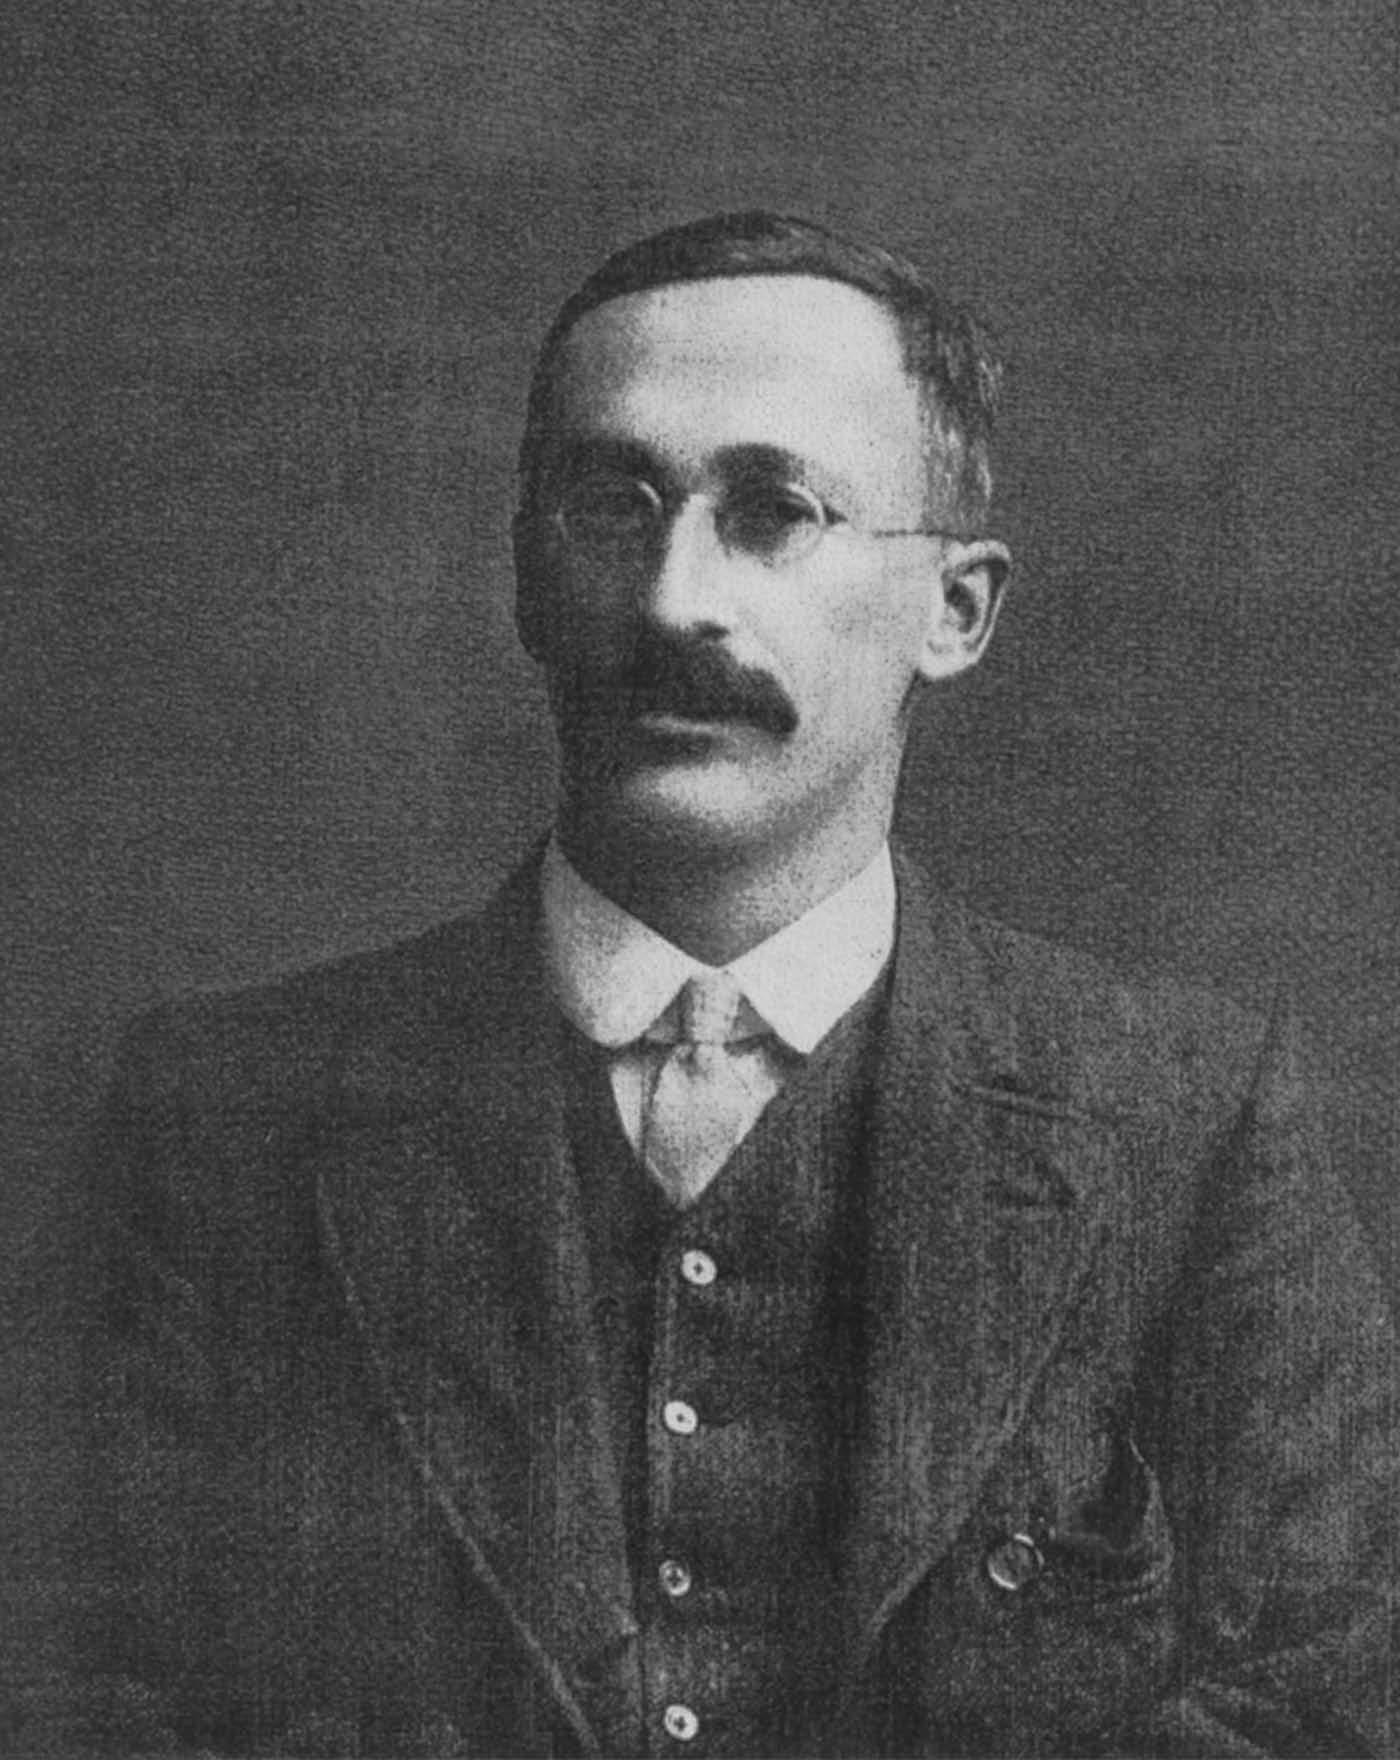
\includegraphics[scale = 0.05]{./images/gosset}}
\vspace{0.75em}


\includegraphics[scale = 0.17]{./images/guinness}
\end{figure}


\column{0.7\textwidth}
\footnotesize
\begin{quote}
``Student'' is the pseudonym used in 19 of 21 published articles by William Sealy
Gosset, who was a chemist, brewer, inventor, and self-trained statistician, agronomer, and designer of experiments ... [Gosset] worked his entire adult life ... as an experimental brewer for one employer: Arthur Guinness, Son \& Company, Ltd., Dublin, St.\ James’s Gate. Gosset was a master brewer and rose in fact to the top of the top of the brewing industry: Head Brewer of Guinness.
\end{quote}

\end{columns}

\end{frame}

%%%%%%%%%%%%%%%%%%%%%%%%%%%%%%%%%%%%%%%%


\begin{frame}
\frametitle{Three Key Sampling Distributions}
Suppose that $X_1, \hdots, X_n \sim \mbox{iid } N(\mu,\sigma^2)$. Then:

	\begin{eqnarray*}
		\left(\frac{n-1}{\sigma^2}\right) S^2&\sim&\chi^2(n-1)\\ \\
		\frac{\bar{X}_n-\mu}{\sigma/\sqrt{n}}&\sim& N(0,1)\\ \\
		\frac{\bar{X}_n-\mu}{S/\sqrt{n}}&\sim&t(n-1)
	\end{eqnarray*}
\end{frame}
%%%%%%%%%%%%%%%%%%%%%%%%%%%%%%%%%%%%%%%%

\begin{frame}
\frametitle{CI for Mean of Normal Distribution, Popn.\ Var.\ Unknown}
Same argument as we used when the variance was known, except with $t(n-1)$ rather than standard normal distribution:
	\begin{eqnarray*}
		P\left(-c \leq \frac{\bar{X}_n-\mu}{S/\sqrt{n}} \leq c \right) &=& 1-\alpha \\ \\ 
		P\left(\bar{X}_n - c \frac{S}{\sqrt{n}} \leq \mu\leq \bar{X}_n +c \frac{S}{\sqrt{n}} \right) &=& 1-\alpha 
	\end{eqnarray*}

\alert{$c =$ \texttt{qt}$(1-\alpha/2, \texttt{df} = n-1)$} 
	$$\boxed{\bar{X}_n \pm \texttt{qt}(1-\alpha/2, \texttt{df} = n-1)\;  \frac{S}{\sqrt{n}}}$$
\end{frame}



%%%%%%%%%%%%%%%%%%%%%%%%%%%%%%%%%%%%%%%%
\begin{frame}
\frametitle{Comparison of CIs for Mean of Normal Distribution}
\framesubtitle{$100\times(1-\alpha)\%$ Confidence Level}
$$\boxed{X_1, \hdots, X_n \sim \mbox{iid } N(\mu, \sigma^2)}$$


\begin{block}{Known Population Std.\ Dev.\ ($\sigma$)}
	$$\bar{X}_n \pm \; \texttt{qnorm}(1-\alpha/2) \; \frac{\sigma}{\sqrt{n}}$$
\end{block}


\begin{block}{Unknown Population Std.\ Dev.\ ($\sigma$)}
$$\bar{X}_n \pm \; \texttt{qt}(1-\alpha/2, \texttt{df} = n-1) \; \frac{S}{\sqrt{n}}$$
\end{block}
\end{frame}
%%%%%%%%%%%%%%%%%%%%%%%%%%%%%%%%%%%%%%%%
\begin{frame}
\frametitle{Standard Error vs.\ Estimator of Standard Error}
\begin{block}{Standard Error}
Recall that the standard deviation of  the sampling distribution of an estimator is called the \emph{\alert{standard error} (SE)} of that estimator.
\end{block}
\begin{block}{Example: Standard Error of the Mean}
$SE(\bar{X}_n) = \sqrt{Var\left(\bar{X_n}\right)} = \sigma/\sqrt{n}$
\end{block}



\begin{alertblock}{Estimator of Standard Error of the Mean} Whereas $\sigma/\sqrt{n}$ \alert{\emph{is}} the standard error of the mean, $S/\sqrt{n}$ is an \alert{\emph{estimator}} of this quantity: $\widehat{SE}(\bar{X_n}) = S/\sqrt{n}$
\end{alertblock}
\end{frame}
%%%%%%%%%%%%%%%%%%%%%%%%%%%%%%%%%%%%%%%%
\begin{frame}
\frametitle{Writing the CIs in terms of Actual and Estimated SE}
\framesubtitle{$100\times(1-\alpha)\%$ Confidence Level}
$$\boxed{X_1, \hdots, X_n \sim \mbox{iid } N(\mu, \sigma^2)}$$

\begin{block}{Known Population Std.\ Dev.\ ($\sigma$)}
	$$\bar{X}_n \pm \; \texttt{qnorm}(1-\alpha/2) \; \alert{SE(\bar{X}_n)}$$
\end{block}

\begin{block}{Unknown Population Std.\ Dev.\ ($\sigma$)}
$$\bar{X}_n \pm \; \texttt{qt}(1-\alpha/2, \texttt{df} = n-1) \; \alert{\widehat{SE}(\bar{X}_n)}$$
\end{block}
\end{frame}
%%%%%%%%%%%%%%%%%%%%%%%%%%%%%%%%%%%%%%%%
\begin{frame}
\frametitle{Comparison of Normal and $t$ CIs}
\begin{table}
\caption{Values of \texttt{qt}$(1-\alpha/2, \texttt{df}=n-1)$ for various choices of $n$ and $\alpha$. }
\begin{tabular}{r|rrrrr|r}
\hline
$n$& 1& 5& 10& 30& 100 & $\infty$\\
\hline
$\alpha = 0.10$&  6.31& 2.02 & 1.81 & 1.70  & 1.66 &1.64\\
$\alpha = 0.05$ & 12.71& 2.57 & 2.23 & 2.04  & 1.98 &1.96\\
$\alpha = 0.01$ & 63.66& 4.03 & 3.17 & 2.75  & 2.63 &2.58\\
\hline
\end{tabular}
\end{table}
\alert{Recall that as $n\rightarrow \infty$, $t(n-1) \rightarrow N(0,1)$}
\vspace{1em}


In a sense, using the $t$-distribution involves making a ``small-sample correction.'' In other words, it is only when $n$ is fairly small that this makes a practical difference for our confidence intervals.
\end{frame}
%%%%%%%%%%%%%%%%%%%%%%%%%%%%%%%%%%%%%%%%


\begin{frame}
\frametitle{Am I Taller Than The Average American Male?}
\framesubtitle{\href{http://www.cdc.gov/nchs/data/series/sr_11/sr11_252.pdf}{\fbox{Source: Centers for Disease Control (pg.\ 16)}}}


\begin{columns}
\column{0.4\textwidth}
\footnotesize
		\begin{tabular}{|lr|}
		\hline
			Sample Mean & 69 inches\\
			Sample Std.\ Dev.\ & 6 inches\\
			Sample Size & 5647 \\
			\hline
			My Height & 73 inches\\
			\hline
		\end{tabular}

\begin{eqnarray*}
\widehat{SE}(\bar{X}_n) &=& s/\sqrt{n}\\
	& =& 6/\sqrt{5647}\\ 
	&\approx& 0.08
\end{eqnarray*}


\column{0.6\textwidth}
Assuming the population is normal,\\
$\boxed{\bar{X}_n \pm \; \texttt{qt}(1-\alpha/2, \texttt{df} = n-1) \; \widehat{SE}(\bar{X}_n)}$
	

\vspace{1em}
\alert{What is the approximate value of \texttt{qt(1-0.05/2, df = 5646)}?} \pause


\vspace{1em}
For large $n$, $t(n-1) \approx N(0,1)$, so the answer is approximately 2
\pause

 \vspace{1em}
\alert{What is the ME for the 95\% CI?} 

\pause $ME \approx 0.16 \implies69 \pm 0.16$

\end{columns}
 


\end{frame}
%%%%%%%%%%%%%%%%%%%%%%%%%%%%%%%%%%%%%%%%

\end{document}
